\documentclass{pnp_article}

\externaldocument{../pus/PusExtension}  % Allows cross-references to Def. Doc.
\externaldocument{../um/PusExtensionUM}   	% Allows cross-references to UM

\begin{document}

\SetDocIssue{0.2}
\SetDocRefNumber{PP-RP-PUX-0001}
\SetDocTitle{CORDET Framework - PUS Extension}
\SetDocSubtitle{Software Verification Report}
\SetDocAuthor{Alessandro Pasetti}
\SetCheckedBy{n.a.}
\maketitle

\maketitle

\newpage
%\listofchanges
\tableofcontents
%\newpage
%\listoffigures
%\newpage
%\listoftables


%==========================================================================================
\section{References}
The documents referenced in this document are listed in table \ref{tab:refdoc}.

\listofreferencedocs{\PxVr}

%==========================================================================================
\section{Introduction}
This document is the software verification report for the PUS Extension of the CORDET Framework. It presents and evaluates the verification evidence collected for the framework at design and implementation level. Table \ref{tab:VerIssues} lists all the verification issues which are addressed in this document. The rightmost column points to the section within the document where each issue is discussed in detail.

The PUS Extension of the CORDET Framework is specified in reference [CR-SP] and its user manual is in reference [CR-UM].

\begin{pnptable}{|>{\raggedright\arraybackslash}p{3cm}|>{\raggedright\arraybackslash}p{8.5cm}|c|}{Verification Issues Addressed in This Document}{tab:VerIssues}{Name & Short Description & Sect.}
Req. traceability & Verify that all requirements are implemented & \ref{sec:svrReqTr} \\
\hline
Req. verification & Verify that all requirements are verified & \ref{sec:svrReqVer} \\
\hline
Static code analysis & Verify that the code is free of statically identifiable bugs & \ref{sec:svrStaticCodeAna} \\
\hline
Code coverage & Verify level of code coverage (statement, branch and condition) achieved through unit-level tests & \ref{sec:svrCodeCov} \\
\hline
Unit tests & Verify that all unit-level tests are successfully executed & \ref{sec:svrUnitLeveTests} \\
\hline
Comment coverage & Verify that all parts of the code are commented & \ref{sec:svrCommCov} \\
\hline
Mem. management & Verify that there are no memory leaks & \ref{sec:svrMemMng} \\
\hline
Schedulability & Verify that the framework supports application- and system-level schedulability analyses & \ref{sec:svrSched} \\
\hline
Software metrics & Verify that the level of complexity of the framework code is acceptable & \ref{sec:svrSwMetrics} \\
\hline
Automatically generated code & Verify that the quality of the automatically generated code used in the framework is adequate & \ref{sec:svrAutoCode} \\
\hline
External libraries & Verify that the qualification levels of the external libraries used by the framework is adequate & \ref{sec:svrExtLib} \\
\hline
\end{pnptable}

%--------------------------------------------------------------------------------------------
\subsection{Framework Constituents}\label{sec:svrConstituents}
For the purposes of assessing the qualification status of the PUS Extension of the CORDET Framework, it is useful to divide its code into the constituent parts listed in table \ref{tab:ConstParts}. The second column in the table identifies the generation method of each component and is one of: (a) 'Reused', if the component is imported into the PUS Extension of the CORDET Framework without changes; (b) 'Generated', if the component is auto-coded; or (c) 'Manual', if the component is developed manually. The third column in the table gives the qualification status of the component which is either 'Qualified', if sufficient verification evidence is already available for the component, or 'To Be Qualified', if the component must be verified within the PUS Extension of the CORDET Framework Project itself.

%--------------------------------------------------------------------------------------------
\subsection{Open Issues}\label{sec:svrOpenIssues}
An \textit{Open Issue} is an issue whose resolution may have an impact on the design or implementation of the framework. The open issues are tracked in the framework's GitHub project.  



\begin{landscape}

\begin{pnptable}{|c|>{\raggedright\arraybackslash}p{3cm}|>{\centering\arraybackslash}p{2cm}|>{\centering\arraybackslash}p{2cm}|>{\raggedright\arraybackslash}p{10cm}|}{PUS Extension of the CORDET Framework Components}{tab:ConstParts}{ID & Description & Gen. Status & Qual. Status & Remarks}
1 & C Libraries & Reused & Qualified & C libraries used by the framework are listed in section \ref{sec:lib} of reference [CR-UM]; they are assumed to be qualified through their extensive use in open software projects \\
\hline
2 & FW Profile Library & Reused & Qualified & This library is provided with a qualification data package which is evaluated in section \ref{sec:svrExtLib} \\
\hline
3 & CORDET Framework Library & Reused & Qualified & This library is provided with a qualification data package which is evaluated in section \ref{sec:svrExtLib} \\
\hline
4 & Configuration Code & Generated & To Be Qualified & Configuration code for the state machines and procedures used in the framework. Its qualification status is evaluated in section \ref{sec:svrAutoCode}. \\
\hline
5 & All Other Code & Manual & To Be Qualified & Manually developed code of the framework \\
\hline
\end{pnptable}

\end{landscape}



%==========================================================================================
\section{Requirement Traceability}\label{sec:svrReqTr} 
The PUS Extension of the CORDET Framework is specified in reference [CR-SP]. The framework is specified in terms of three kinds of requirements:

\begin{itemize}
\item{} \textit{Standard Requirements} which define a desired feature of the framework extension. They are analogous in scope and format to the user requirements of a conventional (non-framework) application.
\item{} \textit{Adaptation Requirement} which define the points where a component offered by the framework extension can be extended by the application developers. In some cases, the definition of an adaptation point is accompanied by the definition of the default options offered by the framework extension for that adaptation point.  
\item{} \textit{Use Constraint Requirements} which define the constraints on how the components offered by the framework extension may be used by application developers.
\end{itemize}

Table \ref{tab:SReqTrace} shows how each Standard Requirement is implemented in the framework code. 

The Adaptation Points are of two kinds: adaptation points which are inherited from the CORDET Framework and new adaptation points which are defined by the PUS Extension. The new adaptation points are those with an identifier of the form Sx. Table \ref{tab:AReqTrace} lists both kinds of adaptation points and shows how each is mapped to code. Note that, in the case of adaptation points which are inherited from the CORDET Framework and are closed by the PUS Extension, the mapping to code takes the form of a pointer to a code-level module where the close-out is done; in the case of new adaptation points, instead, the mapping to code takes the form of a statement explaining how the adaptation point can be closed at code level by an application.

The Use Constraint Requirements are not mapped to code. 


\begin{landscape}
\pnpcsvtable{|l|>{\raggedright\arraybackslash}p{9cm}|>{\raggedright\arraybackslash}p{9cm}|}{Traceability of Standard Requirements to Implementation}{tab:SReqTrace}{Req. ID & Requirement Text & Implementation }{../pus/PusExtensionReq.csv}{\Category-\Id & \Text & \Implementation}

\newpage
\pnpcsvtable{|l|>{\raggedright\arraybackslash}p{9cm}|>{\raggedright\arraybackslash}p{9cm}|}{Traceability of Adaptation Requirements to Implementation}{tab:AReqTrace}{Req. ID & Requirement Text & Implementation }{../pus/PusExtensionReq.csv}{\Category-\Id & \Text & \Implementation}


\end{landscape}




%==========================================================================================
\section{Requirement Verification}\label{sec:svrReqVer} 
The PUS Extension of the CORDET Framework is specified in reference [TsUsp]. The library is specified in terms of:

\begin{itemize}
\item The interfaces it offers to its user application
\item The functional behaviour it offers to its user application
\item The constraints which the user application must satisfy when using the library
\item The performance guaranteed by the library to its user application
\end{itemize}

The constraints are not verified. For the other three items, the following sub-sections show how:

\begin{itemize}
\item Each interface item is exercised in at least one unit-level test
\item Each functional behaviour is exercised in at least one unit-level test
\item Each performance requirement is verified through a timing analysis
\end{itemize}

%------------------------------------------------------------------------------
\chgZB{
\subsection{Methodology}
The objective of this section is to show that each specification item is covered by at least one test case in the Test Suite (see section \ref{sec:TestSuite} of reference [TsUm]). This is done through traceability matrices which associate a test case to each specification item. 

The traceability matrices are built automatically from information embedded within the source code of the test cases. This information is inserted through doxygen custom tag \texttt{@verify}. The doxygen documentation of a test case contrains one or more \texttt{@verify} tags. Each tag in the header file of test case T identifies one specification item which test case T verifies. 

A script processes the header files of the test cases to build the traceability matrices using the information in the \texttt{@verify} tag. These traceability matrices are used to build the tables presented in this section.
}

%------------------------------------------------------------------------------
\chgZB{
\subsection{Verification of User Interface}
Three kinds of interfaces are specified for the PUS Extension of the CORDET Framework in section \ref{sec:userIf} of reference [TsUsp]. Table \ref{tab:VerUI} lists these user interface items and, for each such item, it provides the test cases where the item is verified. Inspection of the table shows that:

\begin{itemize}
\item All user interface item are covered by the test \chgA{campaign}
\item Interface operations which may have both a success and a failure outcome have been validated with both outcomes
\item The library start-up has been validated both when the server starts first and where the server starts first
\item The operations to start and stop the library have been validated on both the server and client side
\end{itemize}


}

%------------------------------------------------------------------------------
\chgZB{
\subsection{Verification of Functional Behaviour}
Functional behaviour is specified through the state machines and procedures defined in reference [TsUsp]. Tables \ref{tab:OpMode} to \ref{tab:FuncBehaviour} list the items verified in each state machine and in each procedure. Inspection of these tables shows that:

\begin{itemize}
\item All state machine states are verified
\item All state machine transitions are verified
\item All procedure nodes are verified
\item All procedure control flows are verified
\end{itemize}
}
\chgA{
In reference [TsUsp] functional behaviour is also captured by a set of Gherkin-style scenarios. The use scenarios are built around features. Each feature covers one aspect of the library functionality. Table \ref{tab:UseCaseVer} associates to each scenario defined in reference [TsUsp] the test case which verifies the behaviour it describes. Inspection of the table shows that all the behaviours defined by the scenarios is modelled and verified in the test cases.

}



%------------------------------------------------------------------------------
\chgZB{
\subsection{Verification of Performance Requirement}
Three performance requirements are formulated in reference [TsUsp]. The first two requirement cover the time to, respectively, send and receive a message across the TCP link. The required message transfer times are TBD. Hence, the requirements are verified by default but it is noted that section \ref{sec:svrExecTimeLibThread} analyses the message transfer times.

The third requirement specifies that the resolution of the command time-out must be 1 ms. This requirement is verified in test case \texttt{S9\_Overrun}.
}


\newpage
\chgA{
\begin{pnptable}{|>{\raggedright\arraybackslash}p{7cm}|>{\raggedright\arraybackslash}p{6cm}|}{Verification of USP Scenarios}{tab:UseCaseVer}{Scenario & Test Cases}
Nominal PUS Extension of the CORDET Framework start-up - server first & \texttt{S1\_ServerStartFirst}, \texttt{C1\_ServerStartFirst} \\
\hline
Nominal PUS Extension of the CORDET Framework start-up - client first & \texttt{S2\_ClientStartFirst}, \texttt{C2\_ClientStartFirst} \\
\hline 
Nominal PUS Extension of the CORDET Framework shutdown - server first &  \texttt{S1\_ServerStartFirst}, \texttt{C1\_ServerStartFirst} \\
\hline
Nominal PUS Extension of the CORDET Framework shutdown - client first &  \texttt{S2\_ClientStartFirst}, \texttt{C2\_ClientStartFirst} \\
\hline 
PUS Extension of the CORDET Framework shutdown Failure & \texttt{PendingCmd} \\
\hline
Forced PUS Extension of the CORDET Framework shutdown & \texttt{PendingCmd} \\
\hline
Fall-back into ERROR state due to connection error & \texttt{S5\_StressTest} \\
\hline
Fall-back into ERROR state due to syntactical error in a command & \texttt{S6\_IllegalCmd}, \texttt{C6\_IllegalCmd} \\
\hline
Fall-back into ERROR state due to syntactical error in an event & \texttt{S7\_IllegalEvt}, \texttt{C7\_IllegalEvt} \\
\hline
Rejection of a request to send a command due to wrong library mode & \texttt{PendingCmd} \\
\hline
Rejection of a request to send a command due to pending command &  \texttt{PendingCmd}, \texttt{FireAndForgetCmd} \\
\hline
Parallel execution of commands of different types & \texttt{S3\_CmdAndEvt}, \texttt{C3\_CmdAndEvt}, \texttt{CmdTimeOut} \\
\hline
Command with command execution event received on time &  \texttt{S3\_CmdAndEvt}, \texttt{C3\_CmdAndEvt} \\
\hline
Command time-out & \texttt{CmdTimeOut} \\
\hline
Fire-and-forget command & \texttt{S3\_CmdAndEvt}, \texttt{C3\_CmdAndEvt}, \texttt{S5\_StressTest} \\
\hline
Rejection of a request to send an event due to wrong library mode & \texttt{SendEvt} \\
\hline
Nominal event send operation & \texttt{S5\_StressTest}, \texttt{S3\_CmdAndEvt}, \texttt{C3\_CmdAndEvt} \\
\hline
\end{pnptable}
}


\chgZB{
\begin{landscape}
\pnpcsvtable{|l|>{\raggedright\arraybackslash}p{4cm}|>{\raggedright\arraybackslash}p{13cm}|}{Verification of User Interface}{tab:VerUI}{Verified Item & Description & Verification Test Cases}{VerUserInterface.csv}{\texttt{\UIName} & \UIDesc & \UIVer}
\end{landscape}

\pnpcsvtable[filter equal={\AAName}{Operational Mode}]{|l|>{\raggedright\arraybackslash}p{10cm}|}{Verification of Operational Mode State Machine}{tab:OpMode}{Test Case & Verified Item}{VerifyInfo.csv}{\texttt{\TestCase} & \Desc}

\pnpcsvtable[filter equal={\AAName}{Out-Going Command}]{|l|>{\raggedright\arraybackslash}p{10cm}|}{Verification of Out-Going Command State Machine}{tab:OutCmd}{Test Case & Verified Item}{VerifyInfo.csv}{\texttt{\TestCase} & \Desc}

\pnpcsvtable[filter equal={\AAName}{Start-Up}]{|l|>{\raggedright\arraybackslash}p{10cm}|}{Verification of Start-Up Procedure}{tab:StartUp}{Test Case & Verified Item}{VerifyInfo.csv}{\texttt{\TestCase} & \Desc}

\newpage
\pnpcsvtable[filter equal={\AAName}{Shutdown}]{|l|>{\raggedright\arraybackslash}p{10cm}|}{Verification of Shutdown Procedure}{tab:Shutdown}{Test Case & Verified Item}{VerifyInfo.csv}{\texttt{\TestCase} & \Desc}

\pnpcsvtable[filter equal={\AAName}{Incoming Event}]{|l|>{\raggedright\arraybackslash}p{10cm}|}{Verification of Incoming Event Procedure}{tab:InEvt}{Test Case & Verified Item}{VerifyInfo.csv}{\texttt{\TestCase} & \Desc}

\pnpcsvtable[filter equal={\AAName}{Incoming Command}]{|l|>{\raggedright\arraybackslash}p{10cm}|}{Verification of Incoming Command Procedure}{tab:InCmd}{Test Case & Verified Item}{VerifyInfo.csv}{\texttt{\TestCase} & \Desc}

\newpage
\pnpcsvtable[filter equal={\AAName}{Functional Behaviour}]{|l|>{\raggedright\arraybackslash}p{10cm}|}{Verification of Functional Behaviour Procedure}{tab:FuncBehaviour}{Test Case & Verified Item}{VerifyInfo.csv}{\texttt{\TestCase} & \Desc}



}

%==========================================================================================
\section{Static Code Analysis}\label{sec:svrStaticCodeAna}
\chgA{
Two forms of static code analysis were done:

\begin{itemize}
\item Compilation of the PUS Extension of the CORDET Framework with the \texttt{clang} compiler with all warnings enabled
\item Compilation with the \texttt{clang} static analyzer (\texttt{scan-build})
\end{itemize}

The \texttt{clang} compiler only reports the following warning: \texttt{clang: warning: treating 'c' input as 'c++' when in C++ mode, this behavior is deprecated}. This warning is reported for all C-language files in the library (the files from the FW Profile Library, see section \ref{sec:lib} of reference [TsUm], and the files generated by the FW Profile Editor, see section \ref{sec:fwSrcCode} of the same document) and is due to the fact that these files are compiled using \texttt{g++/clang++}. This is intentional and the warnings are therefore accepted.

The \texttt{scan-build} reports the following errors:

\begin{itemize}
\item In method \texttt{TerminateOutCmd} a path is identified resulting in a de-reference of a null pointer. Analysis of the code, however indicates this path is not possible by design.
\item In method \texttt{TsTestCaseSerializer::RunTestCase}, three paths are identified leading to a memory leak. In all three cases, however, the path only arise if the test has failed and, under these conditions, the memory leaks are acceptable.
\end{itemize}

Based on the above, it is concluded that no statically detectable issues are present in the code of the PUS Extension of the CORDET Framework.

}





%==========================================================================================
\section{Code Coverage}\label{sec:svrCodeCov}
Code coverage is measured using the \texttt{gcov} tool. The main page of the Doxygen documentation for the PUS Extension of the CORDET Framework gives access to the coverage web page generated by the \texttt{lcov} tool. For convenience, figure \ref{fig:LcovCodeCovReport} shows the summary report from the \texttt{lcov} tool. The coverage information was derived by running the Test Suite (see section \ref{sec:TestSuite} in reference [TsUm]).

\chgZB{
In order to facilitate the assessment of branch coverage information, the following was done:

\begin{itemize}
\item The library source code is compiled with no optimization (compiler option \texttt{-o0}
\item Compilation is done with the \texttt{-fno-exceptions} option to remove handling of exceptions (each exception handler introduces a "hidden" branch in the C++ code). Note that exception handling is not used in the PUS Extension of the CORDET Framework. 
\item The conditions in \texttt{if-clauses} consist of primitive boolean conditions. This means that condition coverage becomes equivalent to decision coverage.
\item In order to achieve coverage of the code configuring the library thread to use the SCHED\_FIFO scheduling policy, the test suite was run under \texttt{sudo}.
\end{itemize}  

The coverage information generated by \texttt{lcov} has been analysed and the entire source code of the PUS Extension of the CORDET Framework has been found to be covered at both statement and decision/condition level with the following exceptions:

\begin{itemize}
\item The destructors of the PUS Extension of the CORDET Framework objects are not covered because these objects are designed to be never destroyed.
\item The branches where function \texttt{HandleErr} is called are not covered because this function is called in response to failures of system calls and these failure conditions cannot be forced.
\item In some cases, the C++ compiler introduces hidden initialization or finalization code which contain branches which are not taken (e.g. in module \texttt{TsInEvtPrFunc}, the definition of a static variable of type \texttt{std::string} introduces hidden initialization and finalization code which contains branches which are not taken during testing).
\item In function \texttt{TsComLibG2}, one branch is unreachable because the Library Shutdown Procedure executes in zero logical execution time (i.e. the guard on the transition from the SHUTDOWN to the FPS in the Operational Mode State Machine will never be false).
\item \chgA{In the \texttt{TsTcpClient::CloseSocket} method, the branch handling the case of the socket being closed before the socket has been created is not covered because it cannot be simulated (it requires the socket creation operation to fail).}
\item In the \texttt{TsTcp::CloseSocket} method, the code clearing the queue of pending packets is not covered because the situation where the socket is closed while packets are still pending \chgA{cannot be easily} modelled by the test suite.
\item In the \texttt{TsTcp::FlushPackets} method, the situation where a packet is rejected in full by the TCP socket is not covered because this situation \chgA{cannot be easily}  modelled by the test suite.
\end{itemize} 




\begin{landscape}
\pnpfigure[scale=0.55]{Summary Coverage Report of \texttt{lcov} Tool}{fig:LcovCodeCovReport}{LcovCodeCovReport.png}
\end{landscape}


}

%==========================================================================================
\section{Unit-Level Tests}\label{sec:svrUnitLeveTests}
The unit level tests are implemented in the Test Suite described in section \ref{sec:TestSuite} of reference [TsUm]. The outcome of running the entire test suite is in the log file \texttt{/log/TestSuite.log}. Inspecton of this log file (also shown in appendix \ref{sec:testSuiteLog}) shows that all test cases in the test suite have been successfully passed.


%==========================================================================================
\section{Comment Coverage}\label{sec:svrCommCov}
The code of the PUS Extension of the CORDET Framework is documented using doxygen comments. The verification of the coverage of these comments is done as follows:

\begin{itemize}
\item Doxygen is configured to issue a warning in case any coding item is not documented
\item It is verified that Doxygen does not issue any warnings
\end{itemize}

The outcome of this verification activity can be checked in file \texttt{/logs/Doxygen.out} in the delivery file which holds the output of the execution of Doxygen.


%==========================================================================================
\section{Memory Management}\label{sec:svrMemMng}
Verification of absence of memory leaks is done at two levels:

\begin{itemize}
\item Statically, each statement resulting in an allocation of memory from the heap is accompanied by a comment which explains where and under which conditions that memory is released
\item Dynamically, \texttt{Valgrind} reports no memory leaks during the execution of the Test Suite for the PUS Extension of the CORDET Framework.
\end{itemize}

Based on these considerations, it is concluded that there are no memory leaks in the PUS Extension of the CORDET Framework.

Note that no measurement has been made of stack usage but it is stressed that the PUS Extension of the CORDET Framework does not make any recursive function calls\footnote{Recursion is used in the FW Profile Library but, in that case, the depth of recursion is the same as the depth of nesting of state machines (see the FW Profile User Manual in reference [FwProf]). Since no nested state machines are used in the TS Communicaton Library, it can be assumed that no recursion is used.}



%==========================================================================================
\section{Schedulability}\label{sec:svrSched}
\chgZB{
The PUS Extension of the CORDET Framework is not a self-standing executable. Hence, it does not make sense to ask whether the library is schedulable \textit{per se}. The more relevant question is: does the library support the analysis of the schedulability of the application within which it is embedded? This question can be split into the following sub-questions:

\begin{itemize}
\item Is the threading model implemented by the library compatible with application-level schedulability analysis?
\item Is the execution time of library code well characterized?
\end{itemize}

The answer to the first question is provided in sections \ref{sec:tsifLibRtCont} to \ref{sec:MutualExcl} of reference [TsUsp] which describe the scheduling concept for the PUS Extension of the CORDET Framework. This is based on a single library thread with cyclical activation at a user-defined priority and on a protection mechanism for shared resources based on ceiling priority. This scheduling mechanism is amenable to static analysis and is therefore compatible withapplication-level schedulability analysis. The remainder of this section is therefore concerned with the second question. The main conclusions are as follows:

\begin{itemize}
\item The execution time of one Library Thread cycle in idle mode (i.e. in the absence of any TCP socket) is below 100 $\mu$sec
\item The execution time of one Library Thread cycle when receiving an event message of size below TS\_TCP\_SOCKET\_READ\_BUF\_SIZE is below 500 $\mu$sec
\item The execution time of an operation initiated by the user application is below 500 $\mu$sec
\item The duration of the period of a library thread cycle is stable to within $\pm$ 0.1 ms 
\end{itemize}

Timing measurements were made in the environment of section \ref{sec:umVerEnviron} of reference [TsUm] with a "no optimization" compilation. In all cases, the call-back functions supported by the library had dummy implementations which only wrote a short message to  \texttt{stdout}. \chgA{The timing measurements have been made on release 0.3 of the PUS Extension of the CORDET Framework. Changes since that release are not believed to have an impact on timing.}

%-----------------------------------------------------------------------------
\subsection{Code Instrumentation}\label{sec:svrCodeInstrumentation}
Characterization of execution times requires measurements of: 

\begin{itemize}
\item The execution time of the library thread
\item The jitter on the release time of the library thread
\item The execution time of user-initiated operations
\end{itemize}

For the third item, only the \texttt{SendCmd} operation was considered since this is clearly yhe most onerous from a CPU point of view. 

Timing measurements were made after having instrumented the library code as shown in figures \ref{fig:CodeInstrSendCmd} and \ref{fig:CodeInstrLibThread}. In both cases, the instrumentation consists of instructions which write either the current time (through function \texttt{GetCurrentTime()}) or the CPU execution time (through function \texttt{clock()}) to \texttt{stdout}.

The output generated by the instrumented code was processed by the \texttt{TimeAnalysis} GNU Octave script. The raw data used for the timing analyses are in the \texttt{docs/octave} directory of the delivery file in files \texttt{timingLocal.csv} (data from local execution of test suite with both server and client on the same machine) and \texttt{timingRemote.csv} (data from execution of test suite with a remote client).

\pnpfigure[scale=0.52]{Code Instrumentation for \texttt{SendCmd} Operation}{fig:CodeInstrSendCmd}{CodeInstrSendCmd.png}

\pnpfigure[scale=0.52]{Code Instrumentation for Library Thread Operation}{fig:CodeInstrLibThread}{CodeInstrLibThread.png}

%-----------------------------------------------------------------------------
\subsection{Execution Time of Library Thread}\label{sec:svrExecTimeLibThread}
Figures \ref{fig:ExecTimeLibThread} and \ref{fig:ExecTimeLibThreadZoom} show the execution time of the library thread on the server side during an execution of the test suite with both server-side library and client-side library residing on the same machine (i.e. using a \texttt{localhost} TCP connection). 

The interval between about cycle 250 and cycle 850 shows a situation where neither commands nor events are exchanged between TS and Connected Device. Here, the execution time of the Library Thread is below 60 $\mu$sec and is mostly well below 50 $\mu$sec. Since the only activities performed by the library thread in this "idle mode" is the polling of the socket for incoming messages and the check on the command time-out, this execution time can be seen as the overhead due to the polling approach selected for the handling of incoming messages. If, for instance, the library tick period were 10 ms, then this overhead would be below 1\%.

The interval between about cycle 250 and cycle 850 covers the first part of the stress test of the test suite. In this scenario, the TS and the Connected Device are sending commands and events to each other at the rate of 1 command/cycle and 1 event/cycle. The commands and events are of small size (order of 100 bytes). Here, the execution time is typically below 200 $\mu$sec with occasional peaks of up to 400 $\mu$secs. In this interval, the Library Thread is primarily busy processing an incoming event. Hence, its execution time is representative of the time required to receive a small event. 

Finally, the interval from about cycle 850 onward covers the second part of the stress test where TS and Connected Device exchange a very large (129 kBytes) command and a very large event (129 kBytes). The execution time is typically 3 ms with several peaks of about 6 ms and a few peaks of up to 15 ms. In this interval, the main task of the Library Thread is the reception of the large event. Nominally, one such event is received in each cycle but in some cases two are received. Detailed inspection of the test results shows that the execution time of around 5-6 ms often corresponds to situations where two large events are received in the same cycle.

The PUS Extension of the CORDET Framework is configured to collect data from the TCP sockets in chunks of 4096 bytes. The reception of one large event therefore requires the collection of about 31 (129/4.096) such chunks. When processing a large incoming message, the Library Thread executes a loop in each cycle of which one chunk of the message is collected. If one assumes that most of the execution time of the Library Thread is used for this loop, then the execution time of one single cycle is about 100 $\mu$sec (3 ms divided by 31 cycles).

If one brings together the findings from the last two paragraphs, one can conclude that the acquisition of one chunk of data from the TCP socket takes between 100 and 200 $\mu$sec.

Figures \ref{fig:ExecTimeLibThreadRemote} and \ref{fig:ExecTimeLibThreadZoomRemote} show again the execution time of the Library Thread. They differ from figures \ref{fig:ExecTimeLibThread} and \ref{fig:ExecTimeLibThreadZoom} because the PUS Extension of the CORDET Framework was on a remote machine. The following considerations apply:

\begin{itemize}
\item The execution time when the Library Thread is idle (neither receiving nor sending messages) is around 50 $\mu$sec with peaks of up to 100 $\mu$sec. This is slightly higher than in the local case. 
\item The execution time when a small event is received is about twice as large as in the local case at about 300 $\mu$sec with one peak of up to 500 $\mu$sec.
\item The execution time when a large event is received is substantially higher with typical values between 3 and 9 ms and peak values of up to 25 ms.
\end{itemize}

With reference to the last bullet, it is noted that, in the second part of the test, when large commands and events are exchanged between server and client, the \texttt{SendCmd} operation may only send one part of a large command. The remainder is buffered and is sent out but the Library Thread. Hence, in this part of the test, the Library Thread on the server side is busy both receiving the large event and sending chunks of the large command. 

%-----------------------------------------------------------------------------
\subsection{Execution Time of User Application Operations}\label{sec:svrExecTimeUserApp}
Among the operations triggered by the user application, the most demanding is the \texttt{SendCmd} operation to send a command. Figures \ref{fig:ExecTimeSendCmdLocal} and \ref{fig:ExecTimeSendCmdRemote} accordingly show the execution time of the \texttt{SendCmd} operation in the "local case" (both server and client residing on the same machine) and in the "remote case" (server and client residing on two different machines).

In the first part of the test (up to about cycle 300 in the two figures), the server side sends a small command of about 100 bytes of size to the client side. In the second part of the test, the server side sends a large command of 129 kBytes of size to the client side.

In the local case (figure \ref{fig:ExecTimeSendCmdLocal}), there is nearly no difference between the two parts of the test: the execution time of the \texttt{SendCmd} operation is around 100 $\mu$sec with peaks of up to nearly 200 $\mu$sec.

In the remote case (figure \ref{fig:ExecTimeSendCmdRemote}), there is a difference between the first part (execution time of less than 200 $\mu$sec) and the second part  (execution time of up to 450 $\mu$sec). 

%-----------------------------------------------------------------------------
\subsection{Stablity of Library Thread Cycle Duration}\label{sec:svrDurLibThreadCycle}
The Library Thread is designed to run cyclically with a period equal to \texttt{tickDur}. The test suite was configured with \texttt{tickDur} equal to 100 ms. Figures \ref{fig:LibThreadCycleDurLocal} and \ref{fig:LibThreadCycleDurRemote} show the actual duration of a library thread cycle. This is centered around 100 $\mu$sec with a jitter of less than 0.1\%.



\pnpfigure[scale=0.48]{Library Thread Execution Time (Local Case)}{fig:ExecTimeLibThread}{ExecTimeLibThread.png}

\pnpfigure[scale=0.46]{Zoom on Library Thread Execution Time (Local Case)}{fig:ExecTimeLibThreadZoom}{ExecTimeLibThreadZoom.png}

\pnpfigure[scale=0.52]{Library Thread Execution Time (Remote Case)}{fig:ExecTimeLibThreadRemote}{ExecTimeLibThreadRemote.png}

\pnpfigure[scale=0.52]{Zoom on Library Thread Execution Time (Remote Case)}{fig:ExecTimeLibThreadZoomRemote}{ExecTimeLibThreadZoomRemote.png}

\pnpfigure[scale=0.46]{\texttt{SendCmd} Execution Time (Local Case)}{fig:ExecTimeSendCmdLocal}{ExecTimeSendCmdLocal.png}

\pnpfigure[scale=0.46]{\texttt{SendCmd} Execution Time (Remote Case)}{fig:ExecTimeSendCmdRemote}{ExecTimeSendCmdRemote.png}

\pnpfigure[scale=0.44]{Duration of Library Thread Cycle (Local Case)}{fig:LibThreadCycleDurLocal}{LibThreadCycleDurLocal.png}

\pnpfigure[scale=0.44]{Duration of Library Thread Cycle (Remote Case)}{fig:LibThreadCycleDurRemote}{LibThreadCycleDurRemote.png}


} % Beginning of schedulability section



%==========================================================================================
\section{Metrics}\label{sec:svrMetrics}
The fist sub-section presents the software metrics. The second sub-section presents the process metrics.

%-----------------------------------------------------------------------------
\chgZB{
\subsection{Software Metrics}\label{sec:svrSwMetrics}
Software metrics were computed with the aim of measuring the complexity of the code. The tool used to compute the software metrics was \texttt{lizard} version 1.14.10. Its output is in the log file \texttt{Metrics.log} in the \texttt{log} directory of the delivery file.

Table \ref{tab:swMetrics} lists the software metrics and their values. The following considerations apply:

\begin{itemize}
\item The metrics refer to the PUS Extension of the CORDET Framework source code exclusive of the \texttt{protobuf} code and of the test suite code
\item \chgAA{No functions with a CCN higher than 10 were found}.
\end{itemize}

\begin{pnptable}{|c|>{\raggedright\arraybackslash}p{8cm}|c|}{\chgA{Software Metrics}}{tab:swMetrics}{ID & Metrics Name & Value}
SM1 & Number of Lines of Codes & 2370 \\
\hline
SM2 & Number of Functions & 218 \\
\hline
SM3 & Average LOC per Function & 7.6  \\
\hline
SM4 & Average Cyclomatic Complexity Number (CCN) & 1.7 \\
\hline
SM5 & Number of Functions with CCN greater than 10 & 1 \\
\hline
\end{pnptable}

}

%-----------------------------------------------------------------------------
\chgZB{
\subsection{Process Metrics}\label{sec:svrProcMetrics}
The process metrics tracked for this project are listed in table \ref{tab:prMetrics}. 

\begin{pnptable}{|c|>{\raggedright\arraybackslash}p{11cm}|c|}{\chgAA{Process Metrics}}{tab:prMetrics}{ID & Metrics Name & Value}
PM1 & Number of Open Issues (see section \ref{sec:svrOpenIssues}) & \chgA{5} \\
\hline
PM2 & Number of Non-Conformances since Release 1.0 (see section \ref{sec:svrNonConformances}) & 0 \\
\hline
PM3 & Number of Requirement Changes since Release 1.0 (see section \ref{sec:svrReqChanges}) & 0  \\
\hline
\end{pnptable}






}

%==========================================================================================
\section{Automatically Generated Code}\label{sec:svrAutoCode}
The specification of the PUS Extension of the CORDET Framework in reference [TsUsp] consists of a behavioural model of the library which is expressed using state machines and procedures (activity diagrams) with the semantics of the \textit{FW Profile}. The FW Profile is a UML profile defined in reference [FwProf]. 

The state machines and procedures of reference [TsUsp] are built within the \textit{FW Profile Editor}. The FW Profile Editor is a web-based tool which supports the definition of state machines and procedures compliant with the FW Profile. The editor includes an auto-coding back-end which generates the C-code which creates and configures the state machines and procedures. The auto-generated modules in the PUS Extension of the CORDET Framework are those with names like \texttt{TsXyzSm} and \texttt{TsXyzPr}, where 'Xyz' is the name of a state machine or procedure. In the PUS Extension of the CORDET Framework project, the generated code is compiled and linked as C++ code. Appendix \ref{sec:svrFwProfEd} gives an overview of the FW Profile Editor.

Use of an auto-coding approach has the following advantages:

\begin{fw_itemize}
\item Guarantee of consistency between specification and implementation 
\item Faster turn-around time 
\item Reduced verification effort 
\end{fw_itemize}

The first advantage follows from the fact that the implementation is directly and automatically derived from the specification. The second advantage follows from the fact that code is generated automatically which is faster than manual development. The gains in verification effort follow from the fact that generated code can be tested more quickly than manually crafted code (because errors are systematic and hence only coding patterns need to be verified). The next sub-section describes the verification approach for the automatically generated code.

%-----------------------------------------------------------------------------------------
\subsection{Verification Approach}
The software implementing the state machines and procedures consist of two parts:

\begin{enumerate}
\item The software in the FW Profile Library which implements the generic state machine and procedure behaviour; and
\item The software generated by the FW Profile Editor implementing the instantiation and configuration code for a state machine or procedure.
\end{enumerate}

The verification approach for the first item is discussed in section \ref{sec:svrExtLib}. For the second item the following considerations apply:

\begin{enumerate}
\item The generated code consists of a linear (no branching) sequence of functions calls; hence one single test provides full coverage of the entire generated code.
\item The functions called by the generated code are configuration functions provided by the FW Profile Library and the order in which they are called is either immaterial or, if it is subject to constraints, their violation leads to errors detected by a built-in consistency check (see next bullet).
\item The FW Profile Library provides functions \texttt{FwSmCheckRec} and \texttt{FwPrCheck} which perform extensive consistency checks on the configuration of, respectively, a state machine or a procedure; these functions detect errors such as omission of a configuration action or execution of a configuration action with invalid parameters. These functions are called as part of the start-up of the PUS Extension of the CORDET Framework (TBC).
\item Implementation errors in the code generation process are likely to result in systematic coding errors triggering major errors in the test suite for the PUS Extension of the CORDET Framework.
\item The test suite for the PUS Extension of the CORDET Framework (see section \ref{sec:svrUnitLeveTests}) covers every state and every transition of every state machine and every node and every branch of every procedure (see section \ref{sec:svrReqVer}. Thus, any configuration errors in a state machine or procedure would be caught by the test suite.
\end{enumerate}

Based on the above, it is concluded that the automatically generated code implementing the configuration of the state machines and procedures of the PUS Extension of the CORDET Framework can be considered to be adequately verified.



%==========================================================================================
\section{External Libraries}\label{sec:svrExtLib}
The PUS Extension of the CORDET Framework uses two external libraries (see section \ref{sec:lib} of reference [TsUm]):

\begin{itemize}
\item The \texttt{protobuf} library from Google
\item The W Profile Library from reference [FwProf]
\end{itemize}

Their qualification status is assessed in the following subsections.

%--------------------------------------------------------------------------------------
\subsection{Qualification Status of \texttt{protobuf} Library}
The \texttt{protobuf} library is also used in other parts of the TALL project and its qualification status is therefore assumed to have already been established to the satisfaction of the TALL system architect. 

%--------------------------------------------------------------------------------------
\subsection{Qualification Status of FW Profile Library}
The FW Profile is a UML Profile for state machines and procedures (activity diagrams). The FW Profile Library provides an implementation for profile-compliant state machines and procedures. The FW Profile state machines and procedures are used in reference [TsUsp] to specify the behaviour of the PUS Extension of the CORDET Framework. The use of the FW Profile Library to code these state machines and procedures has two advantages:

\begin{itemize}
\item It creates a simple and unambiguous link between specification-level artifacts (the state machines and procedures which specify the library behaviour) and implementation-level artefacts (the software modules which implement the specification-level state machines and artifacts).
\item It results in a very compact implementation of the PUS Extension of the CORDET Framework because most of its branching logic is located in the state machines and procedures and this logic is implemented in the FW Profile Library. 
\end{itemize}

The FW Profile Library is publicly available under the Mozilla Public Licence v2. This licence allows the library code to be embedded within the PUS Extension of the CORDET Framework code without imposing any requirements on the latter. In fact, the full code of the FW Profile Library is included in the delivery file of the PUS Extension of the CORDET Framework.

The FW Profile Library is provided with an own qualification data package (downloable from reference [FwProf]) which covers the following items:

\begin{itemize}
\item A set of \textbf{Software Requirements} which formally specify the implementation
\item A set of \textbf{Behavioural Models} which describe the behaviour of the library components
\item An \textbf{Implementation Traceability Matrix} which shows how each requirement is implemented
\item A \textbf{Verification Traceability Matrix} which shows how the implementation of each requirement is verified
\item A \textbf{Validation Traceability Matrix} which justifies each requirement with respect to the intended use of the library
\item A \textbf{Test Suite} with 100\% statement, function, branch, and condition coverage for the entire library implementation (excluding error branches for system calls)
\item \textbf{Doxygen Documentation} covering the entire library source code
\item A \textbf{User Manual} which explains how the library should be used
\end{itemize}

It is also noted that the FW Profile Library has been successfully used in several industrial project.

Based on the above evidence, it is concluded that the FW Profile Library has an adequate quality for use within the PUS Extension of the CORDET Framework.




\newpage
\appendix
%==========================================================================================
\section{FW Profile Editor and Code Generator}\label{sec:svrFwProfEd}
This appendix describes the FW Profile Editor which is used to define the state machines and procedures which specify the behaviour of the PUS Extension of the CORDET Framework and to generate the code of the functions implementing this behaviour.

\subsection{Overview of FW Profile Editor}
The FW Profile Editor allows a user to draw a state machine or a procedure (activity diagram) in a web-based interface accessible from [FwProfEd]. The semantics of the state machines and procedures is that of the FW Profile of reference [FwProf]. Figure \ref{fig:FwProfileEditorScreenshot} shows a screenshot of the FW Profile Editor.

\begin{figure}[htbp]
 \centering
 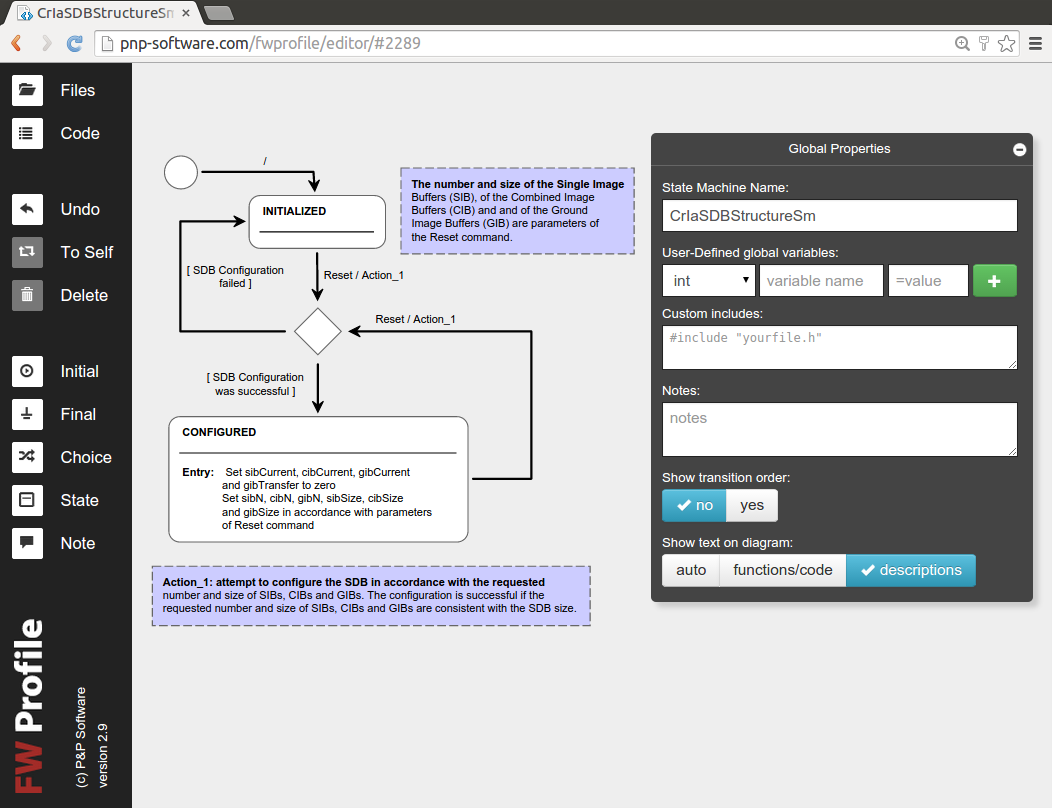
\includegraphics[scale=0.4,keepaspectratio=true]{FwProfileEditorScreenshot.png}
 \caption{Screenshot of the Framework Profile Editor}
 \label{fig:FwProfileEditorScreenshot}
\end{figure}

For each state machine or procedures, the FW Profile Editor offers two "views": the "description view" and the "code view". Users can change between the code view and the description view using a switch in the web-based interface of the editor (see box at the bottom of the "Global Properties" palette in figure \ref{fig:FwProfileEditorScreenshot}).

The two views are illustrated in figures \ref{fig:TsOutCmdSm} and \ref{fig:TsOutCmdSmCode} through the example of the OutCommand State Machine. The description view is used as a specification in the USP of the PUS Extension of the CORDET Framework (see reference [TsUsp]). The actions and guards of the state machine are described through a specification of what they should do. The code view associates code to the actions and guards in the state machine. The code may either take the form of a function name or it may consist of valid C code which directly implements the function. In the example of figure \ref{fig:TsOutCmdSmCode}, the former option. Thus, for instance, \texttt{OutCmdPendingEntry} is the name of a function which implements the entry action of state PENDING in the OutCommand State Machine.


\begin{figure}[H]
 \centering
 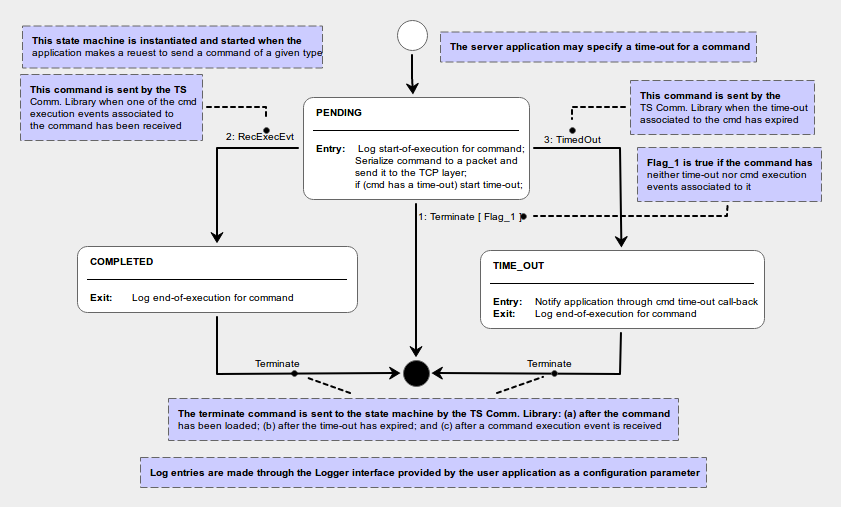
\includegraphics[scale=0.45,keepaspectratio=true]{TsOutCmdSm.png}
 \caption{Description View OutCommand State Machine}
 \label{fig:TsOutCmdSm}
\end{figure}


\begin{figure}[H]
 \centering
 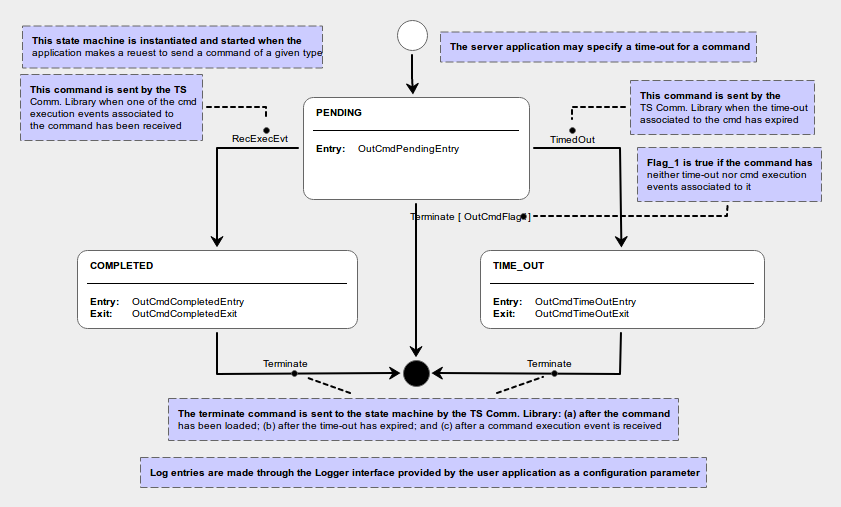
\includegraphics[scale=0.45,keepaspectratio=true]{TsOutCmdSmCode.png}
 \caption{Code View of OutCommand State Machine}
 \label{fig:TsOutCmdSmCode}
\end{figure}

%-----------------------------------------------------------------------------------------
\subsection{Generated Code}
The code generated by the FW Profile Tool for each state machine or procedure consists of three files:

\begin{itemize}
\item A header file which declares the following two items: 
\begin{enumerate}
\item The function to instantiate and configure the state machine or procedure, and
\item Any additional functions implementing actions or guards of the state machine or procedure. 
\end{enumerate}
\item A body file which implements the function which instantiates and configures the state machine or procedure.
\item A dummy \texttt{main} program which instantiates and configures the state machine or procedure and sends a few commands to it. This main program is only intended for demonstration/testing purposes and is not integrated with the application code. 
\end{itemize}

As noted in the previous section, the FW Profile Editor also gives users the option to define the implementation of an action or guard by directly entering the implementing code through the tool interface. In that case, the tool also generates a private (\texttt{static}) function with the code provided by the user. 

The code generated by the FW Profile Editor must be linked with the FW Profile Library (the necessary \texttt{\#include} statements are automatically generated). The library consists of a set of C modules which implement the behaviour of a generic state machine or procedure. Use of this library means that the code generated by the editor only needs to implement the configuration of a state machine or procedure (as opposed to implementing the state machine transition logic or the procedure execution logic). 

For state machines, the configuration code consists of a linear sequence of function calls which "build" the state machine by adding states and transitions and attaching them their attributes (the state and transition actions and the transition guards). Similarly, the configuration of a procedure consists of a sequence of function calls which build the procedure by adding nodes and control flows and to it and attaching them their attributes (the node actions and the control flow guards). 

%-----------------------------------------------------------------------------------------
\subsection{Use of Generated Code}
With the PUS Extension of the CORDET Framework, the auto-generated code is used to create and configure the state machines and procedures. The code must be linked with the manually written code of the PUS Extension of the CORDET Framework but does not need to manually modified in any way.  

The PUS Extension of the CORDET Framework code calls calls the \texttt{Create} function when it needs to instantiate a state machine or procedure. The \texttt{Create} function returns one instance of the state machine or procedure which is fully configured and ready to be used. No further interaction with the generated code is necessary.

%-----------------------------------------------------------------------------------------
\subsection{Summary of Mode of Use of FW Profile Editor}
The FW Profile Editor and its code generator are used as follows in the PUS Extension of the CORDET Framework:

\begin{fw_enumerate}
\item Specification of state machines and procedures using the "description view" of the FW Profile Editor. 
\item Definition of "code view" for the state machines and procedures within the FW Profile Editor. For each action or guard with non-default implementation, a function is defined and its name is entered in the tool. 
\item Generation of code using the FW Profile Editor code generator. For each state machine or procedure, two files are generated (one header file and one body file).
\item For each state machine or procedure, creation of a body file with the implementation of the functions implementing the non-default actions or guards of the state machine or procedure.
\end{fw_enumerate}


%=============================================================================================
\section{Test Suite Log}\label{sec:testSuiteLog}
The listings in this section present the output of the execution of the Test Suite without Valgrind (see listing \ref{lst:testSuite1}) and with Valgrind (see listing \ref{lst:testSuite2}).

\lstinputlisting[label=lst:testSuite1,caption=Test Suite Without Valgrind, language=Tex]{../../../log/TestSuiteRun.log}

\newpage
\lstinputlisting[label=lst:testSuite2,caption=Test Suite With Valgrind, language=Tex]{../../../log/TestSuiteRunWithValgrind.log}




\end{document}